\section{Hardware Design}\label{sec:hw}

\begin{figure*}[htbp]
  \centering
  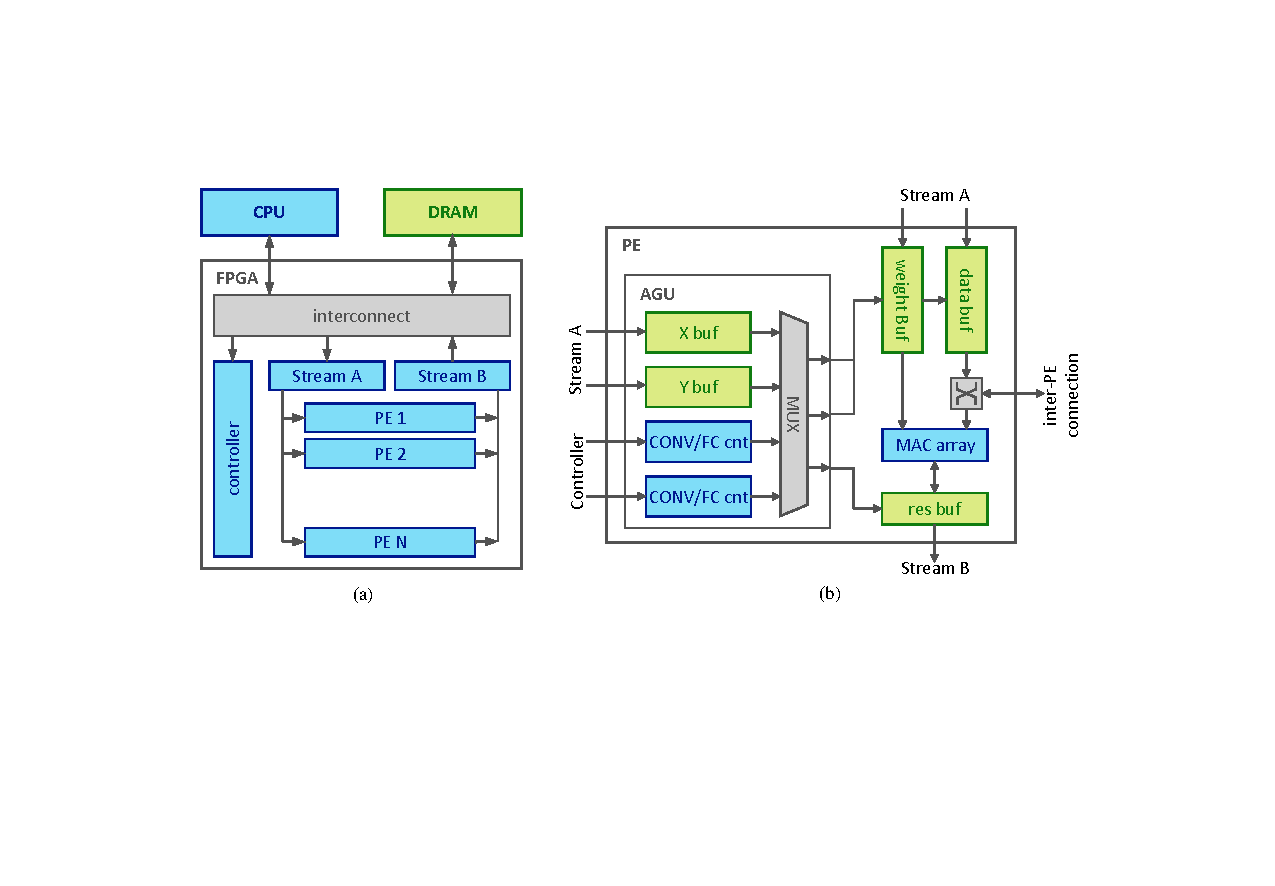
\includegraphics[width=2\columnwidth]{figures/hardware.pdf}
  \caption{The CNN training accelerator architecture. (a) The overall system architecture. (b) The structure of a single PE. }
  \label{fig:arch}
\end{figure*}

In this section, we introduce the hardware design for training CNN with sparse parameters. Especially, we will show architecture support for sparse operations and how this design differ from inference accelerators.

\subsection{Overall Architecture}
Figure~\ref{fig:arch}(a) shows the overall architecture of the hardware design. When the accelerator works, the host CPU sends a mini-batch of training data to the accelerator to process an iteration of training. The accelerator first processes inference on the mini-batch and sends back the result vector to CPU to calculate the loss. After that, the gradient vector of the last layer is given back to the accelerator to do back propagation. This process is iteratively executed until training converges.

External memory are implemented to meet the large storage requirement of training. Compared with inference, the feed-forward results of each layer of the mini-batch should be kept until back propagation is done. Though we use fixed-point data for training, the training on a mini-batch still requires GB level of memory, which is impractical to be stored on-chip. A set of on-chip buffers are implemented to explore the spatial locality of convolution operation and allows fast irregular data access for sparse operations. Details of each PE will be introduced in section~\ref{sec:hw_pe}.

The CNN layers are executed on the hardware layer by layer. For pooling and ReLU layers, the FP, EB and WG phases are all implemented as a pipeline stage after or before PE. Because pooling and ReLU layers has little workload, the functions are implemented as common modules for all the PEs and can be bypassed if necessary. For each layer, the data is first loaded from DDR and is sent to the Upsample/Mask unit. In inference phase, the data is directly issued to corresponding PEs. In back propagation phase, upsampling and mask function is applied on the activation data. Then in each PE, the calculation of the nested loops are processed. Then the results are sent to Pooling/ReLU/Merge unit where the pooling and ReLU function is applied as traditional CNN inference accelerator design. The merge function adds gradient result from different PEs during back propagation phase.

\subsection{PE for Sparse Computation}\label{sec:hw_pe}

To fully take advantage of the sparse weights in training, the hardware should support the following two types of sparse operations:
\begin{itemize}
\item {\bf Operator-sparse}: For FP and EB steps, the activations or errors are multiplied with the sparse weights to get the result feature map or errors. So one of the two operators for multiplication is sparse.
\item {\bf Result-sparse}: For WG steps, the activations are multiplied with the back propagated errors to get the weight gradients. Both the operators of multiplication are dense but the result is sparse.
\end{itemize}

\begin{figure*}[htbp] 
  \centering
  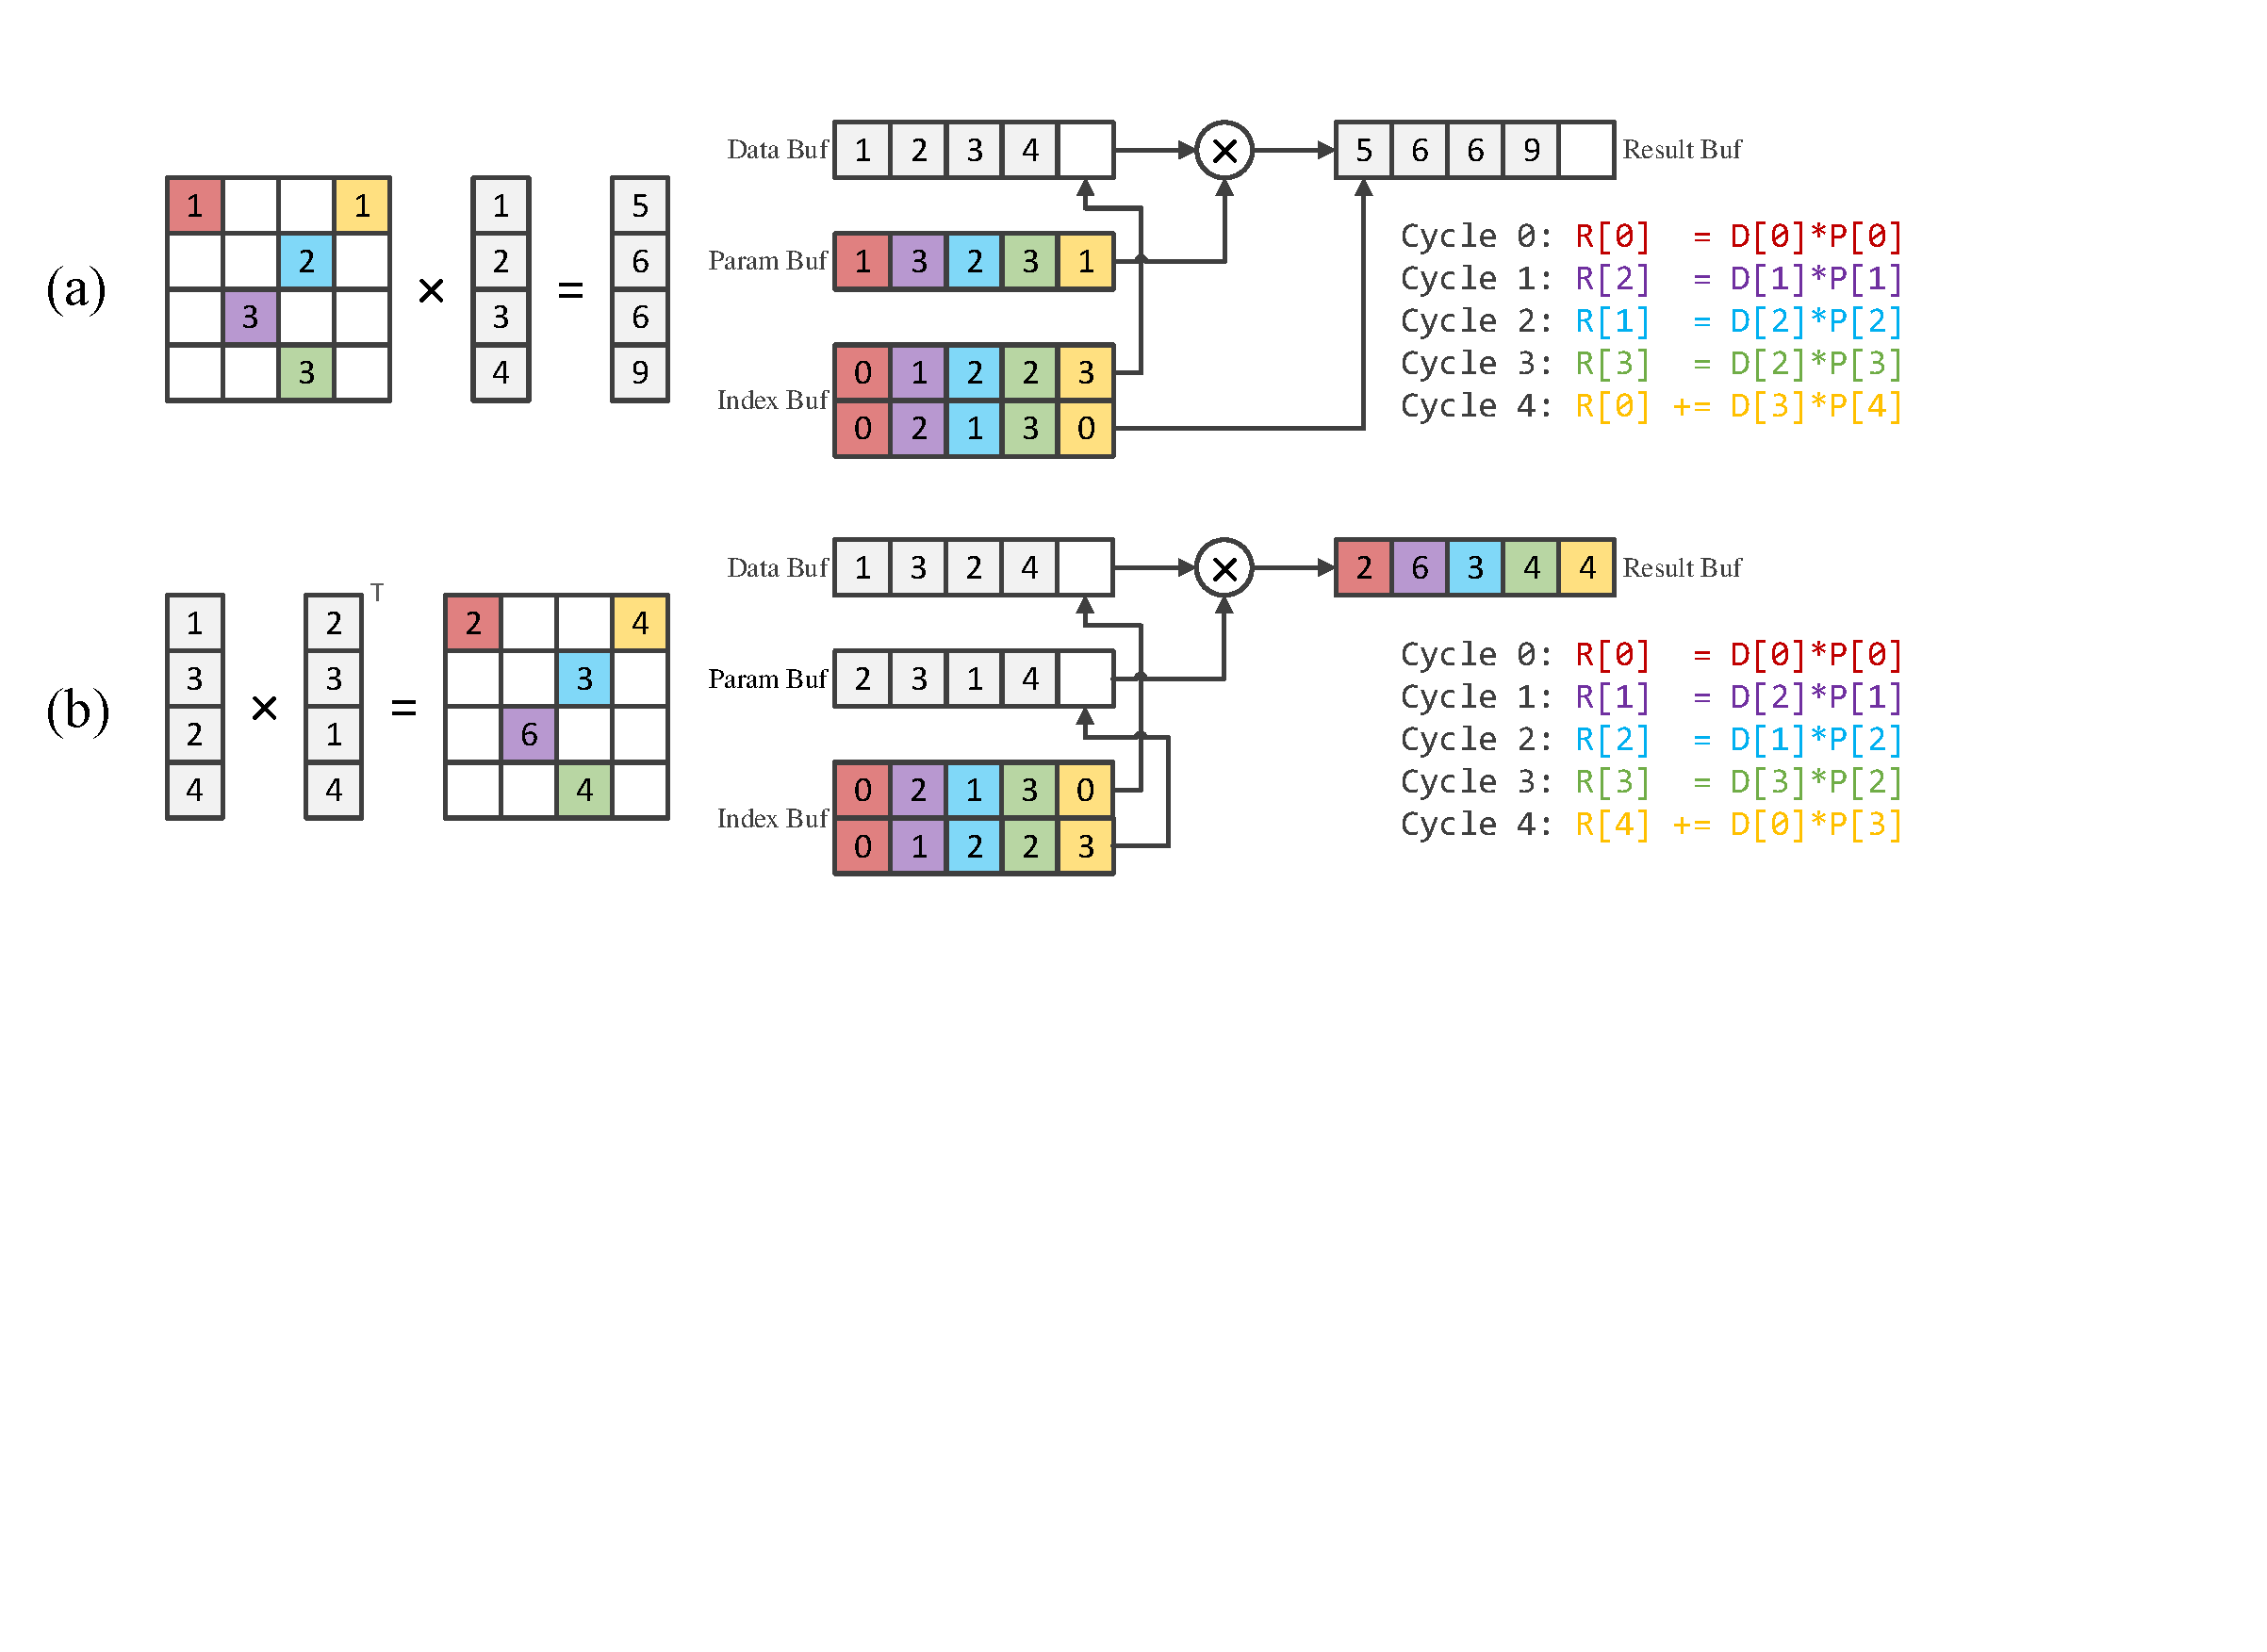
\includegraphics[width=1.8\columnwidth]{figures/sparse_mv.pdf}
  \caption{The hardware behavior for sparse network process. (a) Sparse matrix vector multiplication for inference and calculation of gradient of activations. (b) Vector vector multiplication to calculate the gradient of sparse parameters. }
  \label{fig:spmv}
\end{figure*}

We choose to process the sparse computation in a block manner. In this manner, the hardware can support both of the sparse operation types efficiently. An example of a $4\times 4$ block of fully connected layer executed in a PE is shown in Figure~\ref{fig:spmv}. Each weight matrix element is stored with its relative 2-D position in the block. Each time a pair of index $(x, y)$ is fetched from the index buffer. For inference, as shown in Figure~\ref{fig:spmv}(a), $x$ is used to access the activations in data buffer and $y$ is used to access the result. To calculate the gradient of the sparse parameters, data buffer and parameter buffer store the activation of two adjacent layers. $x$ and $y$ are used to access the buffers respectively. Different PEs work independently on different blocks for higher parallelism.

Note that for the case in Figure~\ref{fig:spmv}(a), changing the order of indexes in index buffer will not change the result, as long as the order of indexes corresponds to that of the parameters. This property is also true for Figure~\ref{fig:spmv}(b). So in NG step, when we need to use a transpose format of the weight matrix, we only need to exchange $x$ and $y$ with a hardware multiplexer and do not need to change the data format in external memory as suggested in Section~\ref{sec:prelim:fc}. 

For CONV layers, as the sparsity is 2-d kernel level structured, the same sparsity is also supplied. If we replace the entries in the matrix with 2-d convolution kernels, each element in vector as a feature map, and scalar multiplication with 2-d convolution, the above example becomes a CONV layer example.

The structure of each PE is shown in Figure~\ref{fig:arch}(b). Similar to the example in Figure~\ref{fig:spmv}, we implement {\bf{DataBuf}} for neuron(feature map), {\bf{ParamBuf}} for weights(convolution kernels) and {\bf{ResBuf}} for neuron(feature map) with on-chip RAM. {\bf{DataBuf}} and {\bf{ParamBuf}} are in simple dual port mode and works in a ping-pong manner by spliting the address space. {\bf{ResBuf}} is implemented with two simple dual port RAMs because accumulation function requires extra RD/WR port.

The detail of the address generation unit(AGU) is shown in Figure~\ref{fig:agu}. AGU implements {\bf{XBuf}} and {\bf{YBuf}} to store the relative index of each weights or convolution kernel within a processing block. We use a multiplexer on the write port of the buffer to support transpose function. For the buffers to be randomly accessed, the X and Y index read from index buffer directly serve as the high bits of RAM addresses, which help to select the channel or neuron to use. An index independent counter helps generate the address sequence to carry out 2-d convolution for CONV layer or scaler multiplication for FC layer. For the buffer to be sequentially accessed, another counter is used generate address sequence.

\subsection{Loop Unrolling Strategy}\label{sec:hw_unroll}
\begin{figure*}[t]
  \centering
  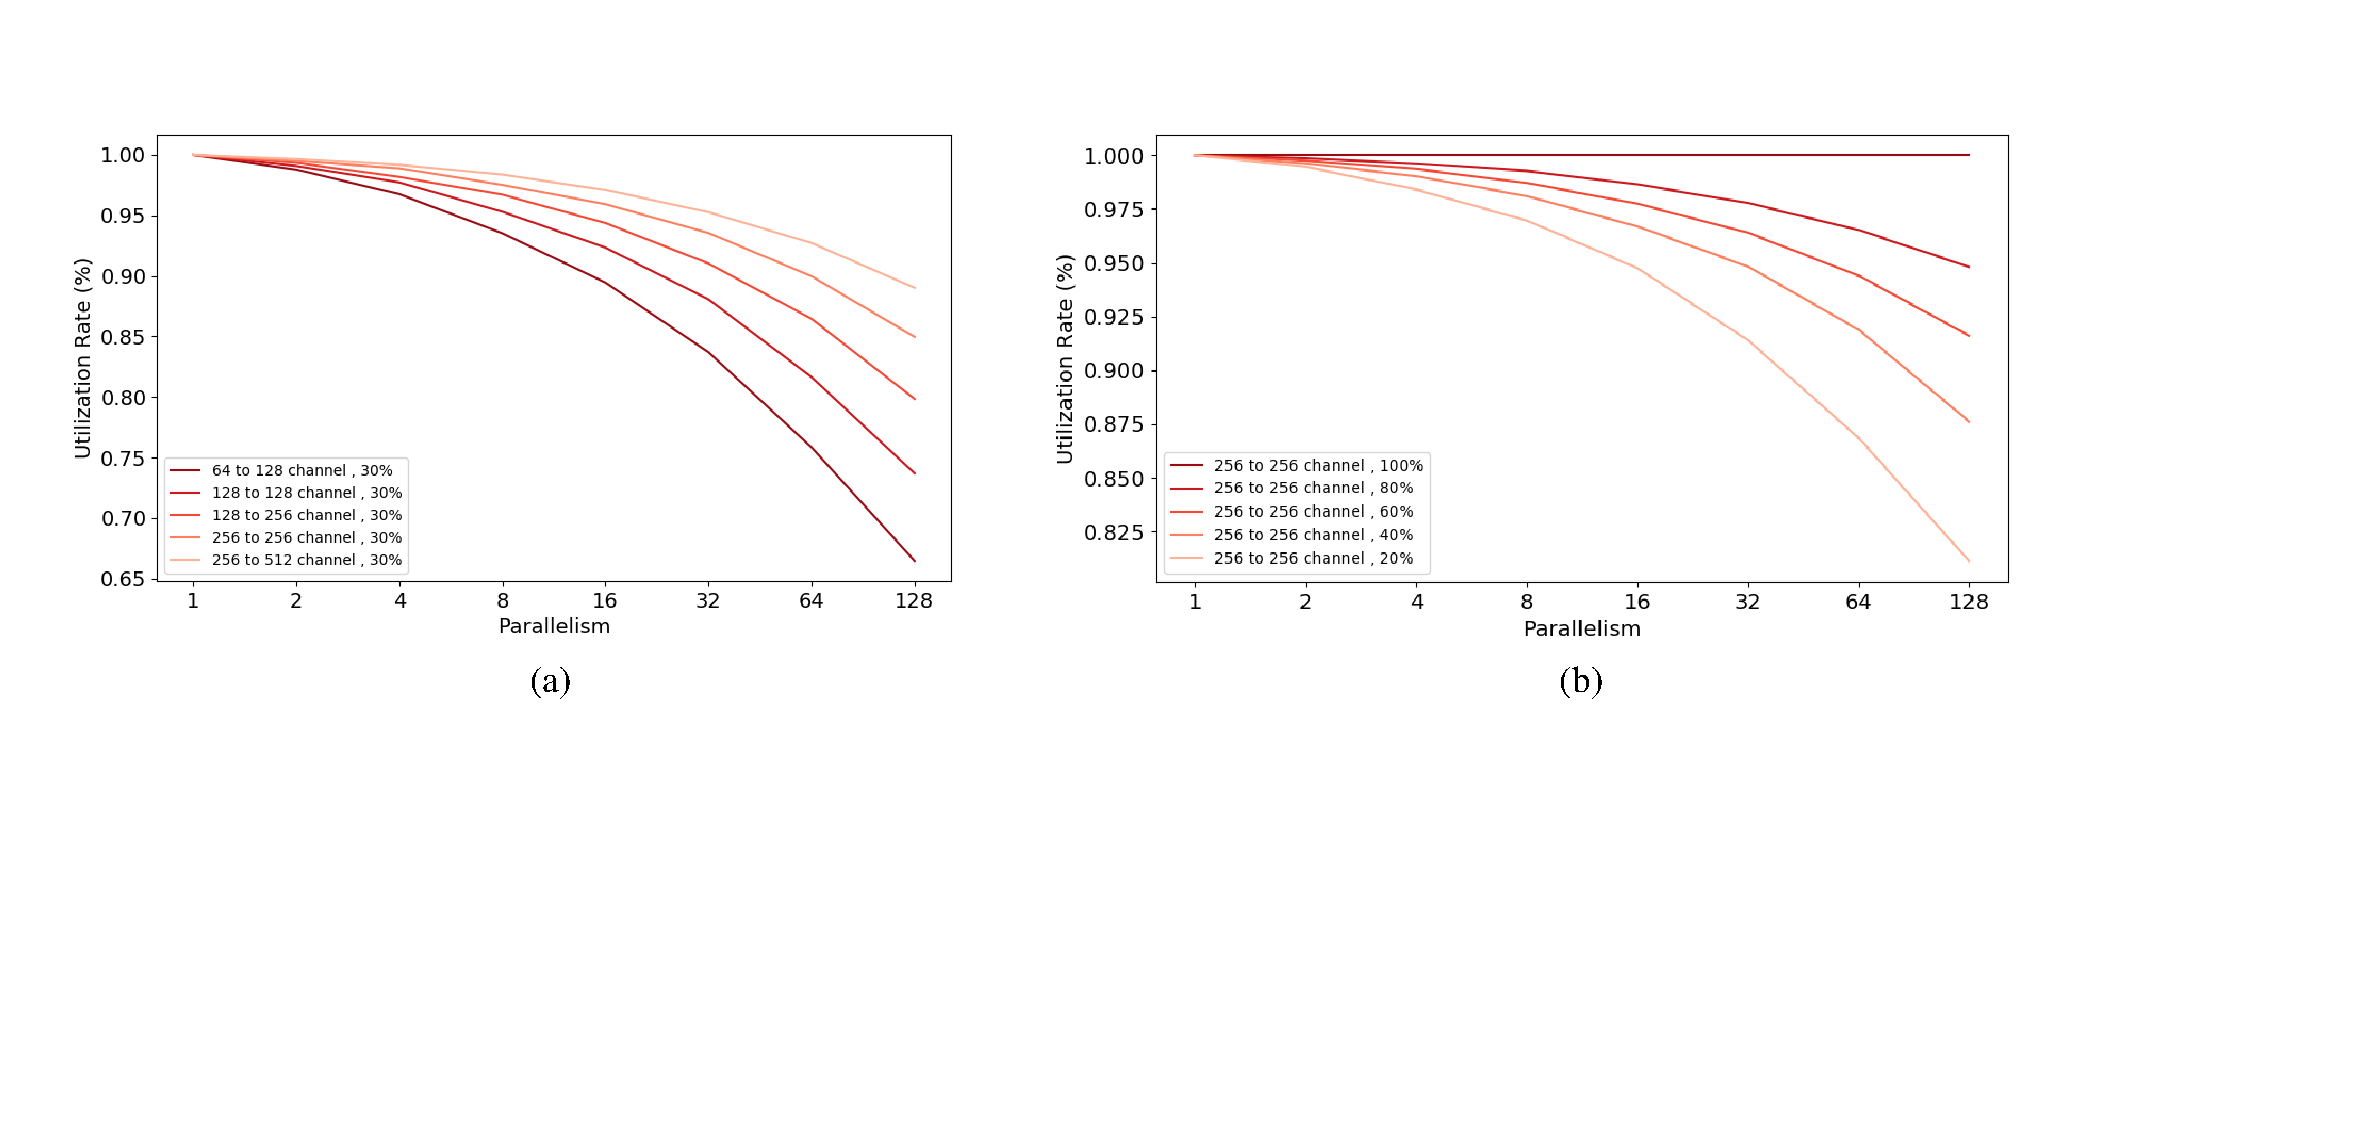
\includegraphics[width=2.0\columnwidth]{figures/util_sim.pdf}
  \caption{Hardware utilization ratio under different sizes of sparse parameters and sparsity. (a) Estimation with a fixed sparsity and different parameter scales. (b) Estimation with a fixed parameter size and different sparsities.}
  \label{fig:util_sim}
\end{figure*}

There is already enough discussions on how to unroll the loops on hardware for CNN inference with dense models~\cite{zhang2015optimizing,mao2017exploring}. But for back propagation and sparse model, the strategy should be different. Here, we analyze different unroll dimensions one by one.

{\bf{Batch}}. Parallelism in batch dimension will not affect hardware design compared with inference accelerator. For training, usually a mini-batch is used in each iteration. So parallelism in batch is always preferred.

{\bf{Layer}}. Parallelize the process of different layers means pipeline different layers. For CNN training, the result of processing one mini-batch is necessary for the next one. So implementing a long pipeline will cause large overhead between the process of adjacent mini-batches. This dimension is not preferred.

{\bf{Input/output channel}}. The unroll parameter in these two dimensions are limited by network sparsity. This is caused by workload imbalance. For example, for a CONV layer, unroll the output channel with M means splitting the workload to M different hardware unit to process in parallel. Because the network is structured sparse, the number of 2-d convolution kernels for each hardware unit to process may different. Some experiments are carried out to show the parallelism affects the hardware utilization ratio as shown in Figure~\ref{fig:util_sim}. In Figure~\ref{fig:util_sim} (a), we suggest that the parameters are uniformly distributed with the density of $30\%$ and varies the size of parameter. It is clear to see that to keep the utilization ratio, we should choose smaller parallelism for a smaller parameter size. In Figure~\ref{fig:util_sim} (b), we keep the parameter size and changes the sparsity. For parameters with less non-zero values, we need to use a smaller parallelism to get the same hardware utilization ratio.

{\bf{Feature map}}. Unrolling in feature map means computing multiple output feature map pixels in parallel. If the output of 2-d convolution is comparable or even smaller than the unroll factor, there will be hardware overhead. For training of CONV layers, the WG steps can be expressed as the 2-d convolution of the input feature map with the gradient of the output feature map. The convolution output size is the same as the convolution kernel, which is usually as small as $3\times 3$. So the unroll factor should be carefully chosen.

{\bf{Convolution kernel}}. Unrolling convolution kernel dimension is faced with the same problem as that of unrolling feature map, not in WG steps, but in FF and NG steps. So the unroll factor should be carefully chosen.

\begin{figure*}[t]
  \centering
  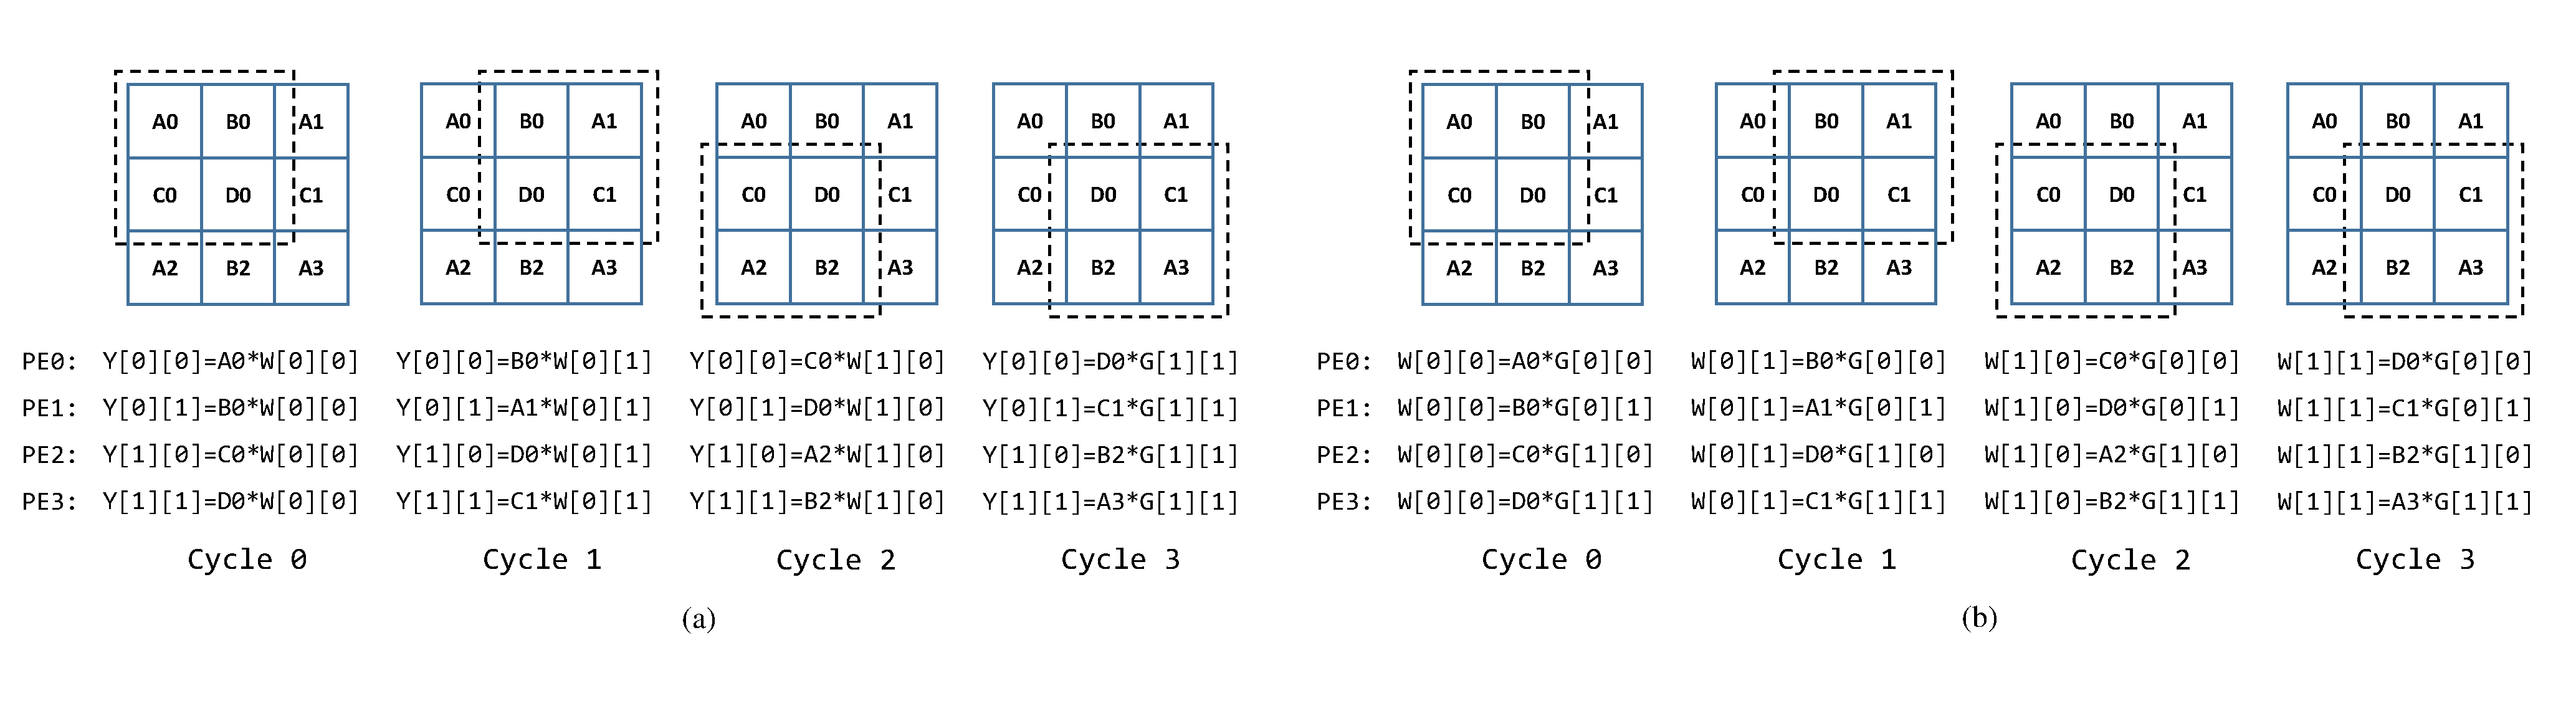
\includegraphics[width=2.0\columnwidth]{figures/mmap.pdf}
  \caption{Example of $2\times 2$ convolution on $3\times 3$ feature map with 4 PEs. The letter in each pixel denotes the PE it belongs to. The number denotes the address it stores in the buffer. The feature map needed for each cycle is marked with the dashed line box. (a) convolution in FF step. (b) convolution in WG step.}
  \label{fig:mmap}
\end{figure*}

So we choose to unroll batch and not implement layer pipeline. Each PE implements $b$ MAC units to process $b$ inputs in parallel. To reduce the channel level parallelism, we explore the possibility of unrolling feature map and convolution kernel dimension in CONV layers. We propose a configurable unroll method between these two dimension. 

For FF and NG steps, we let each $m$ PEs compute $m$ output pixels of a same feature map in parallel. To save on-chip buffer, we split the feature map to $m$ PEs and enables data sharing among them with multiplexers. An example of a $2\times 2$ convolution on a $3\times 3$ feature map with 4PEs are shown in Figure~\ref{fig:mmap}(a). In each cycle, all the PEs fetch the same convolution kernel, multiplies it with a pixel and locally accumulate the result. After 4 cycles, the convolution is done. Note that except for the first cycle, no PE fetches data from its own buffer, which is enabled by data sharing.

For WG step, we let each $m$ PEs fetches $m$ different convolution kernels (in this step is the feature map gradient) and accumulate the result for a same output pixel in parallel. This example is shown in Figure~\ref{fig:mmap}(b). The result are added together when data is written back to external memory. 

\subsection{Data Organization}
\begin{figure*}[htb]
  \centering
  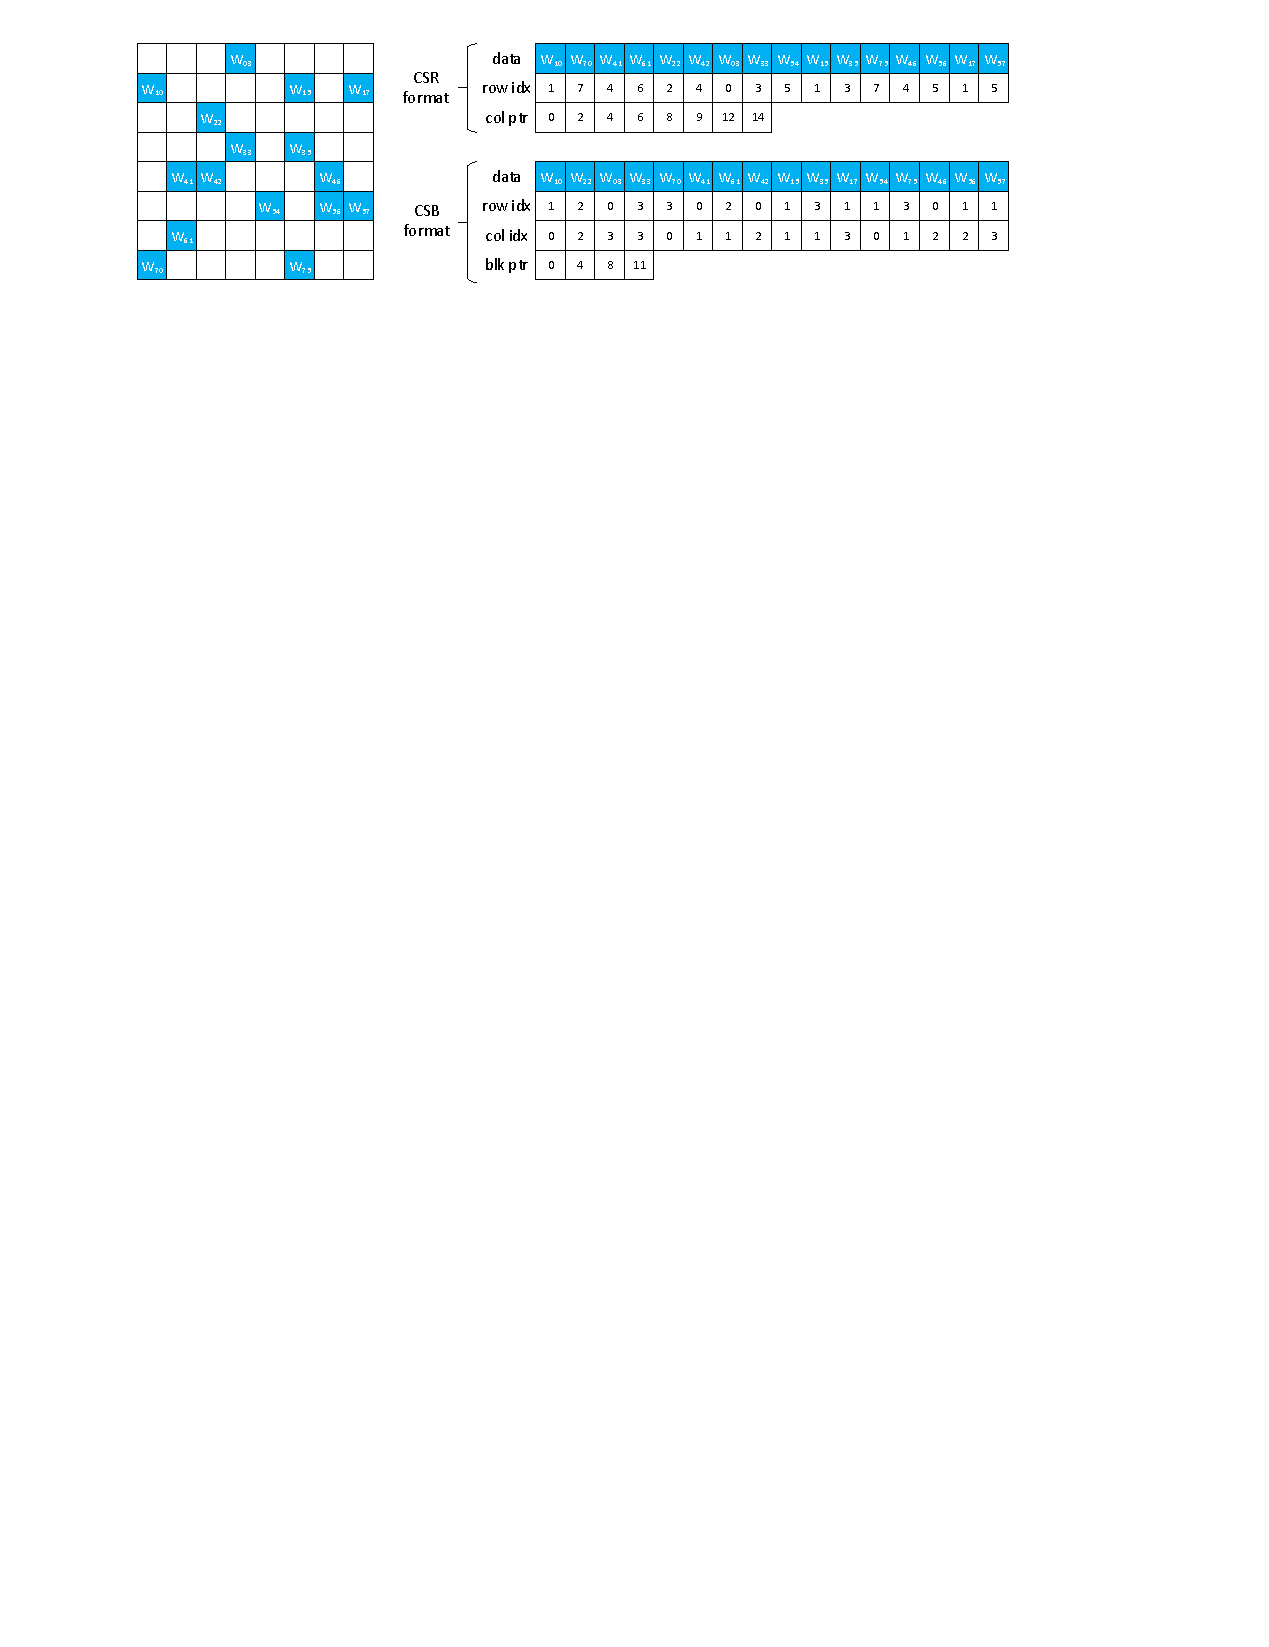
\includegraphics[width=2.0\columnwidth]{figures/csb_new.pdf}
  \caption{Example of different sparse matrix store formats for structured sparse convolution kernels. (a) Compressed Sparse Column(CSC) (b) Compressed Sparse Block(CSB)}
  \label{fig:csb}
\end{figure*}

First, we use the compressed sparsed block (CSB) data format for the sparse weight storage. The sparse weight For fully connected layer, the inference phase and back propagation phase needs to access the parameter matrix in the original version and a transposed version. For convolutional layer, this is similar if we treat it as a 2-D matrix of 2-D convolution kernels. The commonly adopted CSC format, as shown in Figure~\ref{fig:csb}(a) stores data column by column, thus leads to the difficulty in row major access. So we adopt the CSB format~\cite{bulucc2009parallel} where the elements are encoded block by block. In this format, the access direction can be controlled by changing the access order of blocks. This format also fit with the hardware's block-wise process behavior as introduced in section~\ref{sec:hw_pe}. Since the transpose of a single block is achieved in PE level, we can access the sparse weights in both original and transposed format.

Second, we increase the access continuity of feature map by using a $(CHWC_mN)$ storage format. As introduced above, we process the channels in a block manner, and we always process the batch in parallel. So we store a batch of a same pixel continuously. Then, we store each $d$ channels of this pixel together.  $d$ is chosen the same as the corresponding convolution kernel block size of this layer. This requires that the output channel block size of one layer should be the same as the input channel block size of the next. So the memory access burst can reach $d*N*p$ where $p$ is the width to be processed each time, limited by on-chip buffer size and image width. 

\subsection{Scheduling Strategy}

\begin{figure*}[t]
  \centering
  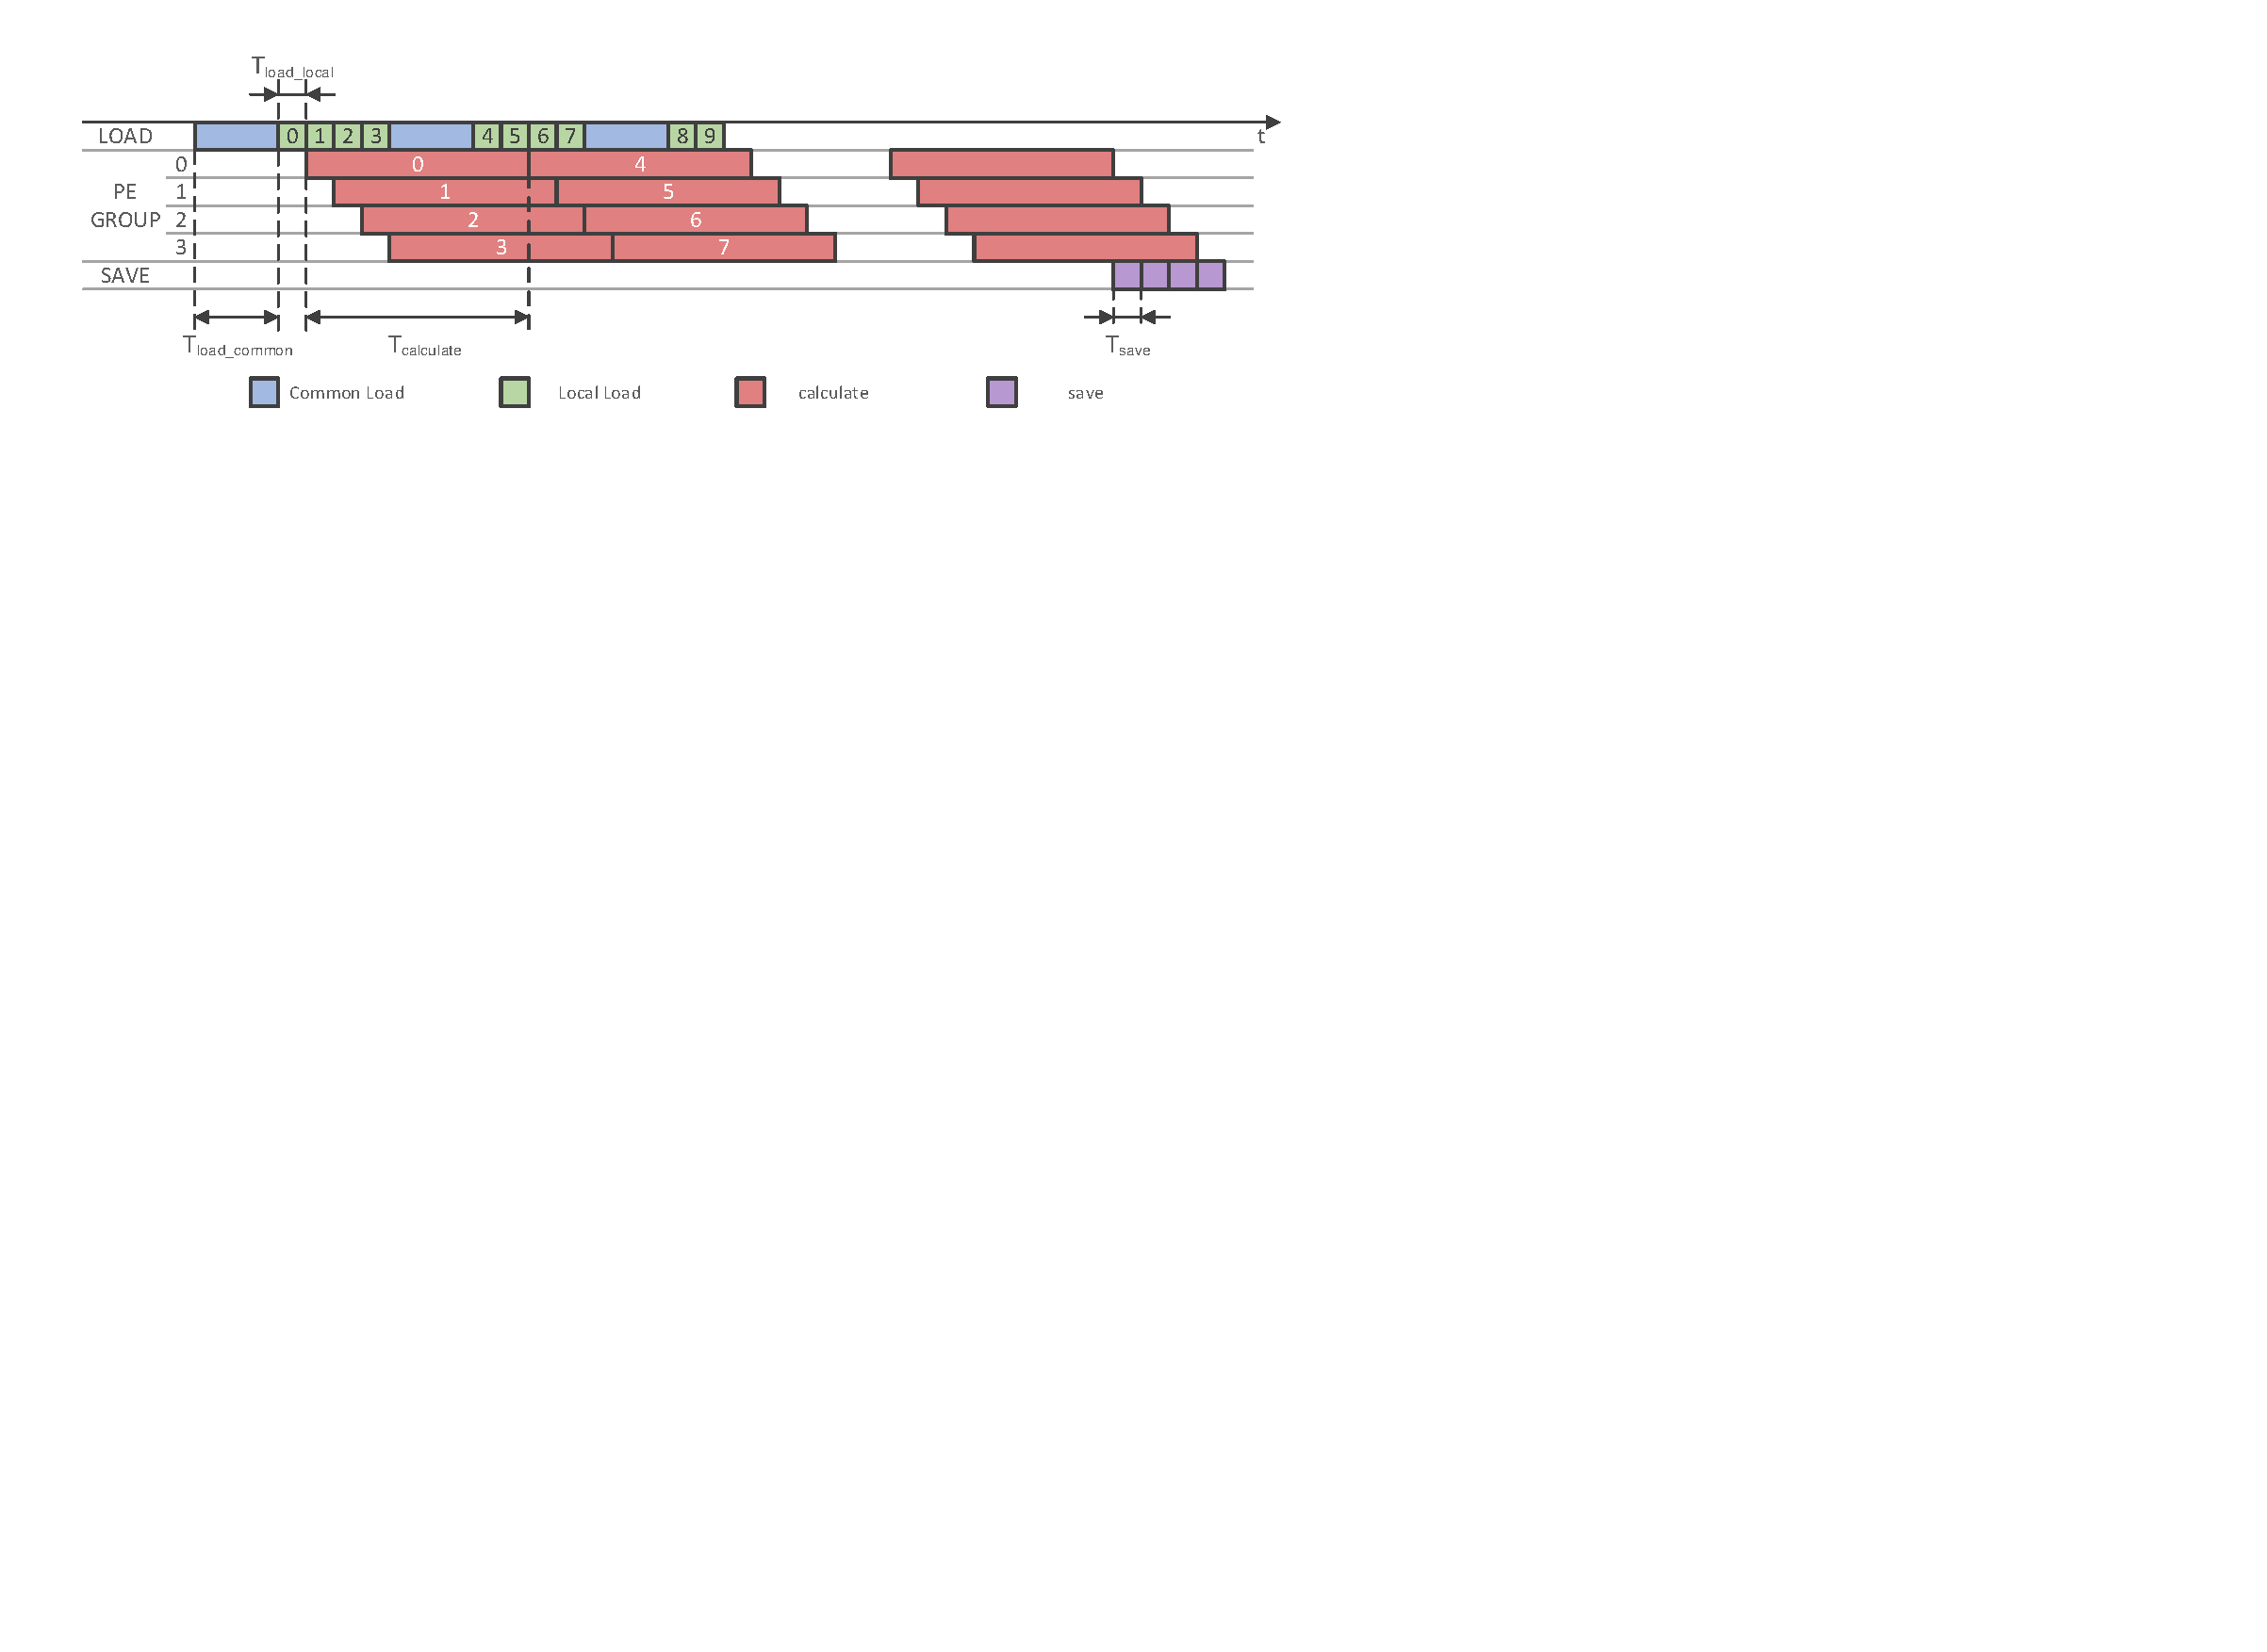
\includegraphics[width=1.8\columnwidth]{figures/schedule.pdf}
  \caption{Example scheduling time line. The number for load local and calculate denote the data dependency}
  \label{fig:sch}
\end{figure*}

As introduced above, each PE will process corresponding computations on a weight block each time. In our scheduling strategy, all the PEs will work with the same input channels/neurons, on different output channels/neurons. They first accumulate the result in ResBuf untill all the input channels are processed, then move on to the next set of output channels. For CONV layers, when all the (input, output) channel pairs are processed, the PEs will move on to the next part of feature map untill the whole feature map is processed. Mainly 4 types of operations are involved in the scheduling strategy.
\begin{itemize}
	\item {{\bf{Common Load}}: Load common data from external memory to all the PEs. In FF and WG steps, this is the common feature maps. In NG step, this is the common feature map gradient.}
    \item {{\bf{Local Load}}: Load local data to a PE or a group of PE. In FF and NG steps, this is the network weights and index. In WG step, this also includes weights buffer.}
    \item {{\bf{Calculation}}: Run a single or group of PE to process a weight block.}
    \item {{\bf{Save}}: Save the result of a single or group of PE to external memory.}
\end{itemize}
Load operation, each PE(PE group), and save operation can work in parallel. Figure~\ref{fig:sch}(a) shows an computation bounded time line example of a system with 4 PE groups. As long as $T_{calc}>T_{load\_common} + T_{load\_local}\times N_{pe}$, the system is computation bounded. Note that in real cases, $T_{calc}$ varies between different PEs and along time as the sparsity is random. $T_save$ can usually be ignored because it appears much less than load.   

